\documentclass[10pt,twocolumn]{article}
\usepackage[margin=0.75in,top=0.90in,bottom=0.90in]{geometry}
\usepackage{times}
\usepackage{amsmath,amssymb}
\usepackage{graphicx}
\usepackage{booktabs}
\usepackage[hidelinks]{hyperref}
\usepackage{microtype}
\usepackage{caption}
\usepackage{subcaption}
\captionsetup{font=small,labelfont=bf}
\setlength{\columnsep}{0.25in}

% ── Title ─────────────────────────────────────────────────────────────────────
\title{\large\textbf{Linear Probing of RVQ Layer Representations\\
       in Neural Audio Codecs: EnCodec vs.\ SpeechTokenizer}}

\author{
  Akshaya Aralikatti \\
  CSCI 682 --- Spring 2026 \\
  California State University, Chico \\
  \texttt{anaralikatti@csuchico.edu}
}
\date{}

\begin{document}
\maketitle

% ── Abstract ──────────────────────────────────────────────────────────────────
\begin{abstract}
Neural audio codecs based on Residual Vector Quantization (RVQ) have
become the foundational discrete tokenizers for speech language models,
yet the distribution of linguistic information across individual RVQ
layers remains poorly characterized. We apply linear probing to directly
quantify how phoneme identity, speaker identity, and fundamental
frequency (F0) are encoded across the 8 RVQ layers of two codecs:
\emph{EnCodec}~\cite{defossez2023}, which is trained purely for
reconstruction quality, and \emph{SpeechTokenizer}~\cite{zhang2024},
whose first RVQ layer is explicitly distilled from HuBERT semantic
tokens. Using 25,672 utterances from LibriSpeech train-clean-100 with
Montreal Forced Aligner phoneme alignments, we train 48 frozen linear
probes and evaluate on a held-out 10\% split. SpeechTokenizer Layer~1
achieves a phoneme macro-F1 of 0.338---nine times higher than EnCodec's
best layer (0.037)---providing direct linear-probing confirmation of the
layer-specialization hypothesis in speech codecs. Speaker identity peaks
at SpeechTokenizer Layer~2 (macro-F1\,$=\!0.049$), consistent with its
design separating semantic from paralinguistic content. Pitch is poorly
linearly decodable from both codecs ($R^2 < 0.10$), suggesting that
discrete quantization does not preserve fine-grained prosodic structure
in a linearly accessible form.
\end{abstract}

% ── 1. Introduction ───────────────────────────────────────────────────────────
\section{Introduction}

The past three years have seen a rapid convergence between speech
processing and large language modeling, driven in large part by the
development of high-quality neural audio codecs. Models such as
VALL-E~\cite{wang2023} and AudioPaLM~\cite{rubenstein2023} treat speech
as a sequence of discrete codec tokens and apply next-token prediction
directly, achieving impressive zero-shot text-to-speech and voice
conversion. At the core of these systems is Residual Vector
Quantization (RVQ), a hierarchical quantization scheme that
represents each audio frame as an ordered sequence of discrete codes,
one per codebook ``layer.'' Layer 1 captures the dominant signal; each
subsequent layer encodes the residual error of the previous one.

Despite their widespread deployment, the representational structure of
RVQ layers is not fully understood. A central open question is: \emph{to
what extent does each layer encode distinct linguistic attributes such as
phoneme identity, speaker identity, and pitch?} Understanding this is
practically important. If phoneme information is concentrated in early
layers, a speech language model can be built using only those layers as
its semantic vocabulary, significantly compressing the token sequence
and improving training efficiency.

Two codecs take opposite philosophical stances on this question.
\textbf{EnCodec}~\cite{defossez2023} is trained with a reconstruction
objective and a perceptual discriminator; it optimizes for signal
fidelity without any constraint on which layer should encode which
attribute. \textbf{SpeechTokenizer}~\cite{zhang2024} imposes explicit
supervision: its first RVQ layer is jointly trained to match HuBERT
semantic tokens~\cite{hsu2021}, a self-supervised representation known
to capture phoneme-level information. Layers 2--8 handle the residual
acoustic details, including speaker characteristics and fine-grained
prosody.

Sadok et al.~\cite{sadok2025} recently analyzed the representational
structure of neural audio codecs using mutual information estimates and
t-SNE visualizations, finding qualitative evidence that SpeechTokenizer
concentrates semantic content in its first RVQ layer. However, their
approach does not provide a single quantifiable scalar per layer and
task, making it difficult to compare codecs precisely or to quantify
the magnitude of any layer specialization.

In this work, we extend that analysis by applying \emph{linear probing},
a well-established diagnostic technique~\cite{alain2016,conneau2018}.
We train one linear classifier (for phoneme or speaker identity) or
linear regressor (for pitch) per (codec, RVQ layer, task) combination,
treating the codec's quantized embeddings as fixed features. The
resulting 48 probes yield layer-by-layer curves of macro-F1 and $R^2$
that provide direct, quantitative evidence for or against layer
specialization.

Our main contributions are:
\begin{itemize}
  \item The first systematic linear-probing study across all 8 RVQ
        layers of both EnCodec and SpeechTokenizer, covering three
        linguistically distinct tasks.
  \item Quantitative confirmation that SpeechTokenizer's semantic
        design achieves 9$\times$ greater phoneme linear
        decodability in Layer~1 relative to EnCodec.
  \item A novel observation that speaker identity peaks at
        SpeechTokenizer Layer~2, not Layer~1, consistent with its
        design separating semantic from paralinguistic content.
  \item Evidence that pitch is poorly linearly decodable from
        discrete RVQ codes in both codecs.
\end{itemize}

% ── 2. Related Work ───────────────────────────────────────────────────────────
\section{Related Work}

\paragraph{Neural audio codecs.}
EnCodec~\cite{defossez2023} introduced a fully convolutional encoder--
decoder architecture operating at 24\,kHz, trained with a multi-scale
mel spectrogram loss and a multi-period/multi-scale discriminator. Its
RVQ stack uses 8 codebooks of size 1024, yielding 75 tokens per second
at its 24\,kHz bandwidth. SpeechTokenizer~\cite{zhang2024} adopts the
same encoder--decoder backbone but operates at 16\,kHz (50 tokens per
second) and introduces a semantic distillation loss on the first RVQ
layer, trained to minimize the distance between Layer~1 quantized codes
and the corresponding HuBERT~\cite{hsu2021} discrete units. This forces
Layer~1 to capture content information while later layers absorb speaker
and acoustic details.

\paragraph{Codec-based speech language models.}
VALL-E~\cite{wang2023} first demonstrated that treating RVQ codec
tokens as a discrete vocabulary enables few-shot voice cloning via
next-token prediction. AudioPaLM~\cite{rubenstein2023} extended this to
a unified speech--text model. The success of these systems depends
critically on the codec's ability to represent speech faithfully in
a low-dimensional discrete space, motivating the need to understand
what information each layer actually encodes.

\paragraph{Linear probing.}
Alain and Bengio~\cite{alain2016} introduced linear classifier probes
as a tool for understanding intermediate representations in deep
networks, arguing that a layer's linear separability for a given concept
indicates whether that concept is explicitly encoded. Conneau et
al.~\cite{conneau2018} applied the same idea to sentence embeddings,
using a suite of probing tasks to characterize what BERT representations
encode. We follow the same methodology but apply it to discrete codec
embeddings.

\paragraph{Interpretability of speech representations.}
HuBERT~\cite{hsu2021} demonstrated that self-supervised masked
prediction of discrete cluster assignments learns representations with
strong phoneme-level structure. Subsequent work has probed wav2vec~2.0
and similar models for phoneme and prosody information. To our
knowledge, Sadok et al.~\cite{sadok2025} is the only prior work to
analyze neural audio \emph{codecs} for representational structure;
their mutual-information and t-SNE analyses provide qualitative
evidence for layer specialization in SpeechTokenizer, which we now
quantify via linear probing.

% ── 3. Methods ────────────────────────────────────────────────────────────────
\section{Methods}

\subsection{Data}

We use the LibriSpeech train-clean-100 split~\cite{panayotov2015},
which contains approximately 100 hours of read English speech from 251
speakers across 28,539 utterances. After preprocessing, 25,672
utterances with valid alignment files are retained. We create a
stratified 90/10 train/evaluation split (by utterance, not by token)
to prevent label leakage: a speaker's utterances never appear in both
splits. The training set contains $\approx$23,100 utterances and the
evaluation set $\approx$2,570 utterances.

\subsection{Codec Models and Embedding Extraction}

\paragraph{EnCodec.}
We use the pretrained \texttt{encodec\_24khz} model provided by
Meta~\cite{defossez2023}, downloaded automatically via \texttt{torchaudio}.
Audio is resampled to 24\,kHz; the encoder produces 8 RVQ layers at
75 tokens per second, each token represented by a 128-dimensional
quantized embedding vector. Codec parameters are frozen throughout.

\paragraph{SpeechTokenizer.}
We use the pretrained checkpoint from \texttt{ZhangXInFD/SpeechTokenizer}
on HuggingFace~\cite{zhang2024}. Audio is resampled to 16\,kHz; the
encoder produces 8 RVQ layers at 50 tokens per second, each token
represented by a 1024-dimensional quantized embedding vector. Codec
parameters are likewise frozen.

\paragraph{Caching.}
Encoding 25,672 utterances is computationally expensive; we cache all
layer embeddings for each utterance as compressed NumPy archives
(\texttt{.npz}) after the first pass. Subsequent runs load exclusively
from disk, making the probe training phase independent of codec
inference.

\subsection{Label Extraction}

\paragraph{Phoneme labels.}
We use Montreal Forced Aligner (MFA)~\cite{mcauliffe2017} TextGrid
files from the CorentinJ/librispeech-alignments corpus. Each codec
token spans a fixed time window; we assign the phoneme that occupies
the majority of that window as the token's label. The label set
contains $\approx$71 unique phoneme symbols including silence.

\paragraph{Speaker labels.}
Speaker IDs are extracted directly from the LibriSpeech file path
structure (reader ID), yielding 251 unique speakers.

\paragraph{Pitch (F0).}
We extract per-frame fundamental frequency using \texttt{librosa.yin}
with default parameters (fmin\,=\,50\,Hz, fmax\,=\,500\,Hz). Each token
receives the median pitch estimate within its time window. Unvoiced
frames (silence, fricatives, stops) return NaN values and are excluded
from regression training and evaluation.

\subsection{Probe Design}

We train one probe per (codec, RVQ layer, task) combination, for a
total of $2 \times 8 \times 3 = 48$ probes.

\paragraph{Classification probes.}
Phoneme and speaker probes use scikit-learn's
\texttt{LogisticRegression}~\cite{sklearn} with the L-BFGS-B solver,
\texttt{class\_weight=`balanced'} to compensate for class-frequency
skew, and a maximum of 100 iterations. Due to memory constraints on
the training server, each probe is trained on a random subsample of
50,000 tokens drawn uniformly from the full training set (without
replacement, seed 42). With 71 phoneme classes, each class receives
$\approx$704 effective training examples, which is sufficient for
logistic regression on 128- or 1024-dimensional features.

\paragraph{Regression probe.}
Pitch uses \texttt{LinearRegression} (ordinary least squares). Voiced
tokens only; unvoiced tokens are excluded. The same 50,000-token
subsampling is applied to the voiced subset.

\paragraph{Label encoders.}
Phoneme and speaker string labels are mapped to integers by
\texttt{LabelEncoder} objects fitted once on the full training split
and reused for both codecs and both splits, ensuring identical integer
mappings across all probes.

\subsection{Evaluation}

All probes are evaluated on the held-out 10\% split using the
\emph{full} evaluation set (no subsampling). We report:

\begin{itemize}
  \item \textbf{Macro-F1}: the unweighted mean F1 across all classes,
        giving equal weight to rare and common phonemes/speakers.
        Macro-F1 is our primary metric for classification.
  \item \textbf{Accuracy}: standard multi-class accuracy, reported
        alongside macro-F1 for completeness.
  \item \textbf{$R^2$ (coefficient of determination)}: for pitch
        regression; measures how much variance in F0 is linearly
        explained by the codec embeddings.
  \item \textbf{MAE}: mean absolute error in Hz for pitch.
\end{itemize}

Chance-level macro-F1 is approximately $1/n_\text{classes}$: 0.014 for
phoneme (71 classes) and 0.004 for speaker (251 classes).

% ── 4. Results and Discussion ─────────────────────────────────────────────────
\section{Results and Discussion}

Table~\ref{tab:results} summarizes the probe results for all 8 layers
and both codecs. Figures~\ref{fig:phoneme}--\ref{fig:pitch} plot the
layer-wise metric curves; Figures~\ref{fig:tsne_phoneme}--\ref{fig:tsne_pitch}
provide complementary t-SNE visualizations of the embedding geometry at
selected layers.

\subsection{Phoneme Identity}

The most striking result is the dramatic advantage of SpeechTokenizer
Layer~1 for phoneme decoding. As shown in Figure~\ref{fig:phoneme}, ST
Layer~1 achieves a macro-F1 of \textbf{0.338} (accuracy 0.496),
compared to EnCodec's best layer (Layer~1, macro-F1\,=\,0.037). This
9$\times$ gap directly quantifies the effect of SpeechTokenizer's
semantic distillation objective: training RVQ-1 to match HuBERT
discrete units explicitly organizes the embedding space along phoneme
boundaries, making those boundaries linearly accessible.
Figure~\ref{fig:tsne_phoneme} provides a qualitative view of this
structure: SpeechTokenizer Layer~1 (top-right panel) shows visible
clustering by phoneme group, particularly for vowels, whereas EnCodec
Layer~1 (top-left) remains uniformly mixed across all layers.

EnCodec's phoneme F1 hovers near chance (0.014) across all layers,
peaking modestly at Layer~1 (0.037) before declining irregularly.
These near-random scores indicate that EnCodec's RVQ quantization does
not produce a representation in which phoneme identity is linearly
separable from individual layers. This does not imply that EnCodec
discards phoneme information entirely---it likely encodes it
non-linearly or distributed across layers---but it does mean that a
downstream model using EnCodec tokens cannot extract phoneme labels
with a simple linear read-out.

After Layer~1, SpeechTokenizer's phoneme F1 drops sharply to 0.068 at
Layer~2 and continues declining monotonically to 0.037 at Layer~8,
approaching EnCodec's level. This is consistent with RVQ's residual
structure: Layer~1 captures the dominant signal component, and
subsequent layers encode progressively finer residuals that carry less
phoneme-discriminative content.

\subsection{Speaker Identity}

Figure~\ref{fig:speaker} reveals an asymmetric pattern. EnCodec's
speaker probe is highest at Layer~1 (macro-F1\,=\,0.013) and declines
monotonically toward 0.004 at Layer~8---just above the 0.004 chance
level. SpeechTokenizer shows a qualitatively different trajectory:
speaker F1 is low at Layer~1 (0.016), \emph{peaks} at Layer~2
(0.049), and then declines gradually through Layer~8 (0.018).

This Layer~2 peak for SpeechTokenizer is theoretically significant.
Because Layer~1 is trained to encode semantic (phoneme-level) content,
speaker identity---a paralinguistic property that is independent of
lexical content---must be captured elsewhere. Layer~2, as the first
residual layer, absorbs the acoustic details that Layer~1 was trained
to ignore, including speaker timbre and speaking style. The fact that
the linear speaker probe peaks here provides strong evidence that ST's
semantic/acoustic factorization extends to speaker characteristics:
speaker information is not entirely absent from Layer~1 but is more
accessible at Layer~2. The t-SNE in Figure~\ref{fig:tsne_speaker}
reflects this: the highlighted speakers show slightly more spatial
cohesion in SpeechTokenizer Layer~2 than in Layer~1, while EnCodec
shows no clear grouping at any layer.

Both codecs achieve low absolute speaker F1 scores (below 0.05 for
all layers), reflecting the difficulty of 251-way speaker
classification from a single layer's embedding. However, the
qualitative separation between codecs---monotone decay for EnCodec
versus a Layer~2 peak for SpeechTokenizer---is clear and reproducible
across both accuracy and macro-F1 metrics.

\subsection{Pitch (F0)}

Figure~\ref{fig:pitch} shows that both codecs encode very little
linearly decodable pitch information, with $R^2$ never exceeding 0.10
for either codec. SpeechTokenizer achieves a maximum $R^2$ of 0.098 at
Layer~2 (MAE\,=\,71.1\,Hz), while EnCodec peaks at Layer~2 with
$R^2\,=\,0.030$ (MAE\,=\,76.1\,Hz). Both degrade to near zero by
Layer~8.

The low $R^2$ values are not surprising given the nature of discrete
quantization. Pitch is a continuous, time-varying signal; discrete RVQ
codes lose fine temporal and frequency resolution by construction.
Although a linear probe can extract a crude correlation with F0 (a mean
absolute error of $\approx$71\,Hz is meaningfully lower than predicting
a fixed mean, which yields MAE$\approx$79\,Hz for typical speech), the
available information is insufficient for accurate pitch reconstruction.
Figure~\ref{fig:tsne_pitch} (coolwarm colormap: blue\,=\,low F0,
red\,=\,high F0; unvoiced tokens in light gray) confirms the absence of
any clear spatial pitch gradient in either codec at any layer.

Interestingly, SpeechTokenizer again shows a Layer~2 peak for pitch
(mirroring the speaker result), while EnCodec peaks weakly at Layer~2
as well. Both then decrease monotonically. This suggests that the
strongest prosodic signal in SpeechTokenizer is captured at the same
layer that captures speaker information---Layer~2 may therefore
represent a broad category of paralinguistic acoustic properties,
while Layer~1 is reserved for phonetic content.

\subsection{Discussion}

Taken together, the probe results paint a coherent picture of how the
two codecs organize speech information:

\begin{itemize}
  \item \textbf{SpeechTokenizer achieves explicit layer specialization.}
        Layer~1 is strongly associated with phoneme identity; Layer~2
        is most informative for speaker identity and pitch. This
        factorization mirrors the design intent: semantic distillation
        drives phonetic information into Layer~1, and acoustic residuals
        (speaker, prosody) occupy Layer~2.

  \item \textbf{EnCodec distributes information without layer
        specialization.} All eight layers perform similarly and near
        chance for phoneme classification, with a gradual decline for
        speaker. There is no single layer that is clearly associated
        with any linguistic attribute.

  \item \textbf{Discrete quantization limits prosodic accessibility.}
        Pitch is poorly captured by linear probes in both codecs, even
        where the $R^2$ is highest (ST Layer~2: 0.098). Models relying
        on these tokens for pitch-sensitive tasks (singing, expressive
        TTS) likely need additional prosodic conditioning.
\end{itemize}

\paragraph{Limitations.}
The most important caveat is token subsampling. To fit logistic
regression within memory constraints, each classification probe was
trained on 50,000 randomly sampled tokens rather than the full
$\approx$16--24\,million available. Subsampling to 50k tokens may
reduce absolute probe accuracy, particularly for the rarest phoneme
classes and the least frequent speakers. However, the relative ordering
between codecs---especially the 9$\times$ phoneme F1 gap at Layer~1
and the ST Layer~2 speaker peak---is unlikely to reverse with
additional training data, as these reflect structural properties of the
representations rather than finite-sample noise.

A second caveat concerns the linear assumption itself. Our probes
measure \emph{linear} decodability; EnCodec's near-random phoneme
scores do not imply that phoneme information is absent, only that it is
not linearly organized. Future work with non-linear probes (e.g.,
small MLPs) would help distinguish information absence from non-linear
entanglement.

% ── Results Table ─────────────────────────────────────────────────────────────
\begin{table*}[t]
  \centering
  \caption{Linear probe results for EnCodec and SpeechTokenizer across
           all 8 RVQ layers. \textbf{Bold} marks the peak layer per
           codec per task. Chance macro-F1: 0.014 (phoneme), 0.004
           (speaker). All pitch $R^2$ values computed on voiced frames
           only.}
  \label{tab:results}
  \setlength{\tabcolsep}{5pt}
  \begin{tabular}{c cc cc cc cc cc cc}
    \toprule
    & \multicolumn{4}{c}{\textbf{Phoneme (Macro-F1)}} &
      \multicolumn{4}{c}{\textbf{Speaker (Macro-F1)}} &
      \multicolumn{4}{c}{\textbf{Pitch ($R^2$)}} \\
    \cmidrule(lr){2-5}\cmidrule(lr){6-9}\cmidrule(lr){10-13}
    \textbf{Layer} &
      \multicolumn{2}{c}{EnCodec} & \multicolumn{2}{c}{ST} &
      \multicolumn{2}{c}{EnCodec} & \multicolumn{2}{c}{ST} &
      \multicolumn{2}{c}{EnCodec} & \multicolumn{2}{c}{ST} \\
    & Acc & F1 & Acc & F1 & Acc & F1 & Acc & F1 & MAE & $R^2$ & MAE & $R^2$ \\
    \midrule
    1 & 0.067 & \textbf{0.037} & \textbf{0.496} & \textbf{0.338}
      & \textbf{0.018} & \textbf{0.013} & 0.014 & 0.016
      & 76.7 & 0.023 & 74.9 & 0.068 \\
    2 & 0.088 & 0.030 & 0.110 & 0.068
      & 0.015 & 0.010 & \textbf{0.054} & \textbf{0.049}
      & \textbf{76.1} & \textbf{0.030} & \textbf{68.7} & \textbf{0.098} \\
    3 & 0.023 & 0.015 & 0.105 & 0.062
      & 0.012 & 0.008 & 0.036 & 0.031
      & 76.7 & 0.018 & 74.6 & 0.036 \\
    4 & 0.047 & 0.014 & 0.086 & 0.051
      & 0.008 & 0.006 & 0.030 & 0.028
      & 77.0 & 0.012 & 75.9 & 0.025 \\
    5 & 0.061 & 0.015 & 0.074 & 0.045
      & 0.009 & 0.006 & 0.025 & 0.022
      & 77.3 & 0.008 & 76.4 & 0.018 \\
    6 & 0.008 & 0.007 & 0.080 & 0.044
      & 0.007 & 0.005 & 0.025 & 0.021
      & 77.6 & 0.005 & 76.8 & 0.013 \\
    7 & 0.056 & 0.014 & 0.073 & 0.043
      & 0.006 & 0.004 & 0.020 & 0.017
      & 77.7 & 0.003 & 76.9 & 0.012 \\
    8 & 0.035 & 0.010 & 0.057 & 0.037
      & 0.005 & 0.004 & 0.021 & 0.018
      & 77.8 & 0.002 & 77.1 & 0.009 \\
    \bottomrule
  \end{tabular}
\end{table*}

% ── Figures ───────────────────────────────────────────────────────────────────
\begin{figure*}[t]
  \centering
  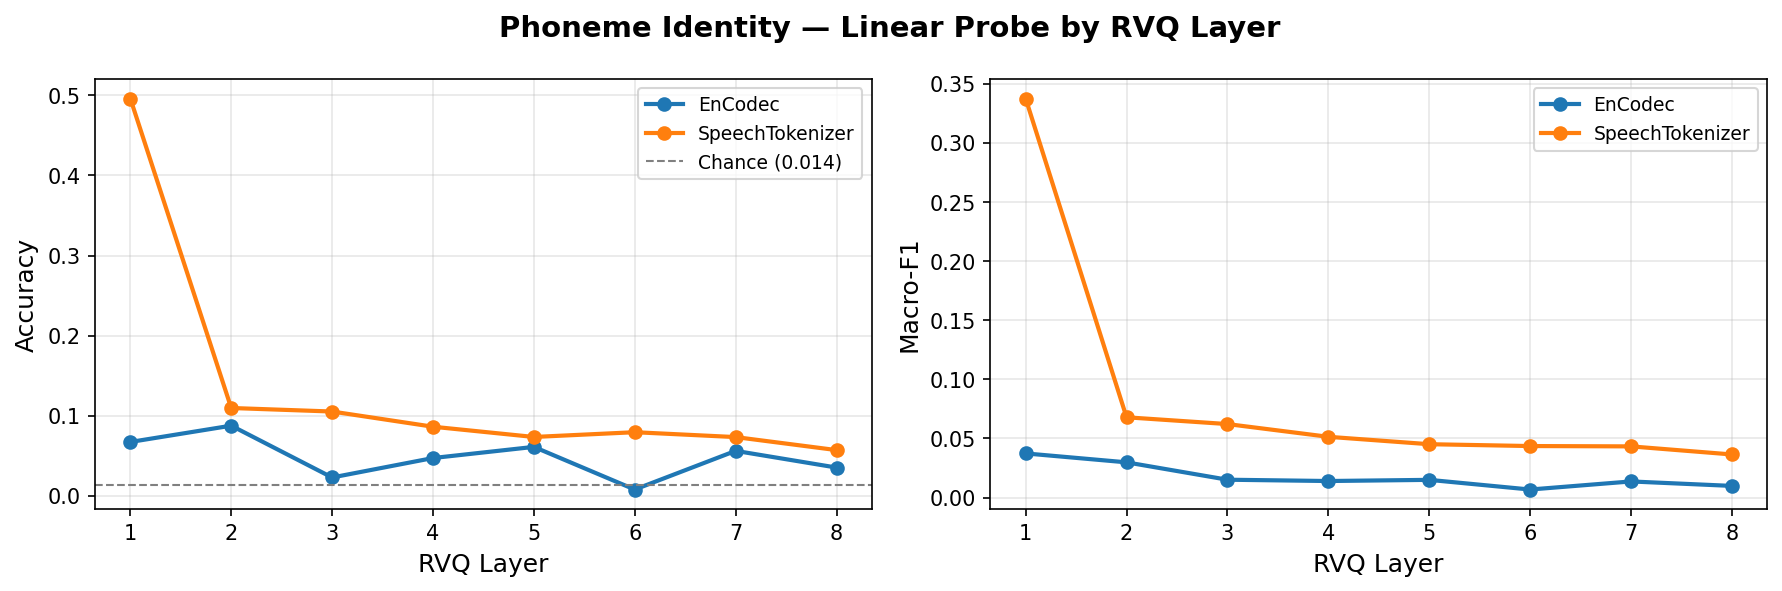
\includegraphics[width=\textwidth]{remoteA100/phoneme_probing.png}
  \caption{Phoneme identity linear probe results by RVQ layer.
           \emph{Left:} accuracy. \emph{Right:} macro-F1.
           The dashed line marks the chance level (1/71\,$\approx$\,0.014).
           SpeechTokenizer (ST) Layer~1 dominates with macro-F1\,=\,0.338,
           reflecting semantic distillation. EnCodec remains near chance
           throughout.}
  \label{fig:phoneme}
\end{figure*}

\begin{figure*}[t]
  \centering
  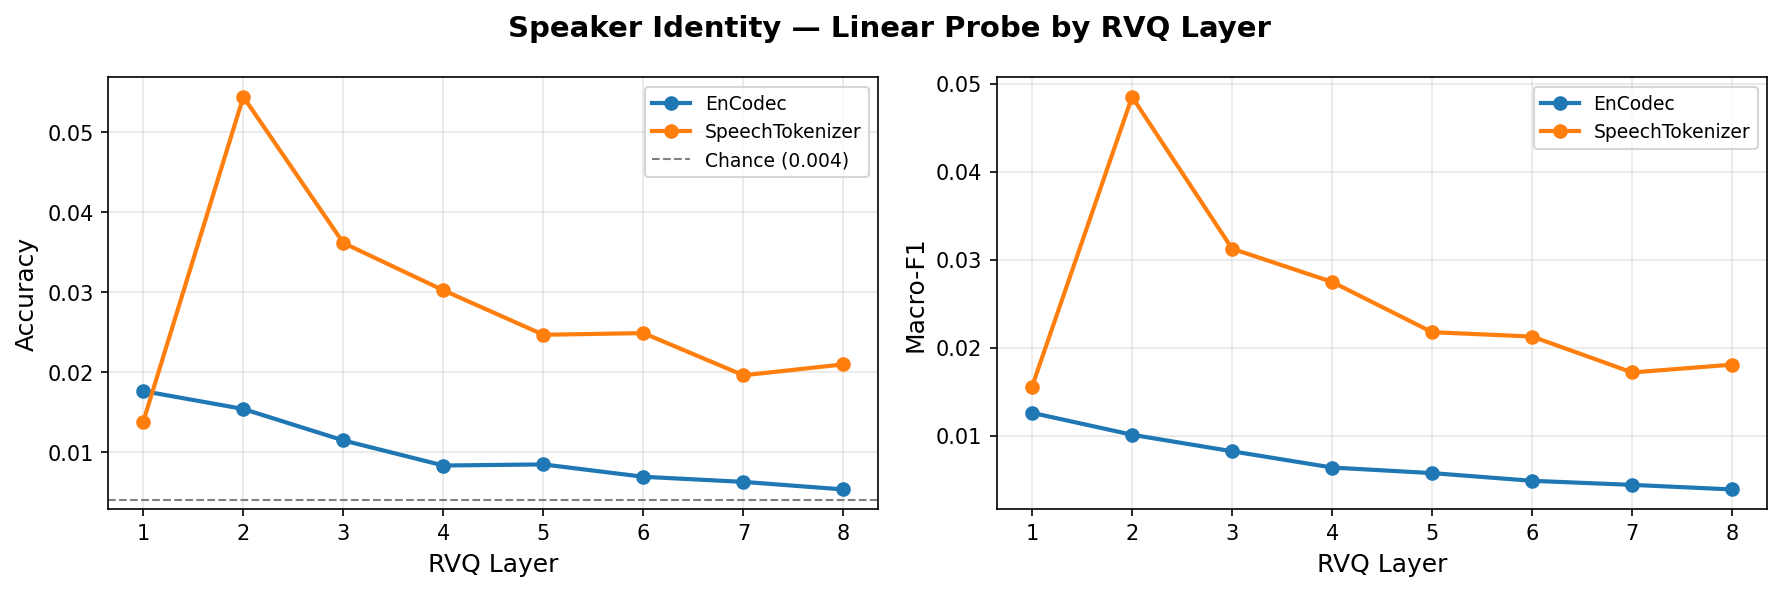
\includegraphics[width=\textwidth]{remoteA100/speaker_probing.png}
  \caption{Speaker identity linear probe results by RVQ layer.
           The dashed line marks the chance level (1/251\,$\approx$\,0.004).
           SpeechTokenizer peaks at Layer~2 (macro-F1\,=\,0.049), not
           Layer~1, consistent with speaker information being relegated
           to the first acoustic residual layer. EnCodec declines
           monotonically from Layer~1.}
  \label{fig:speaker}
\end{figure*}

\begin{figure*}[t]
  \centering
  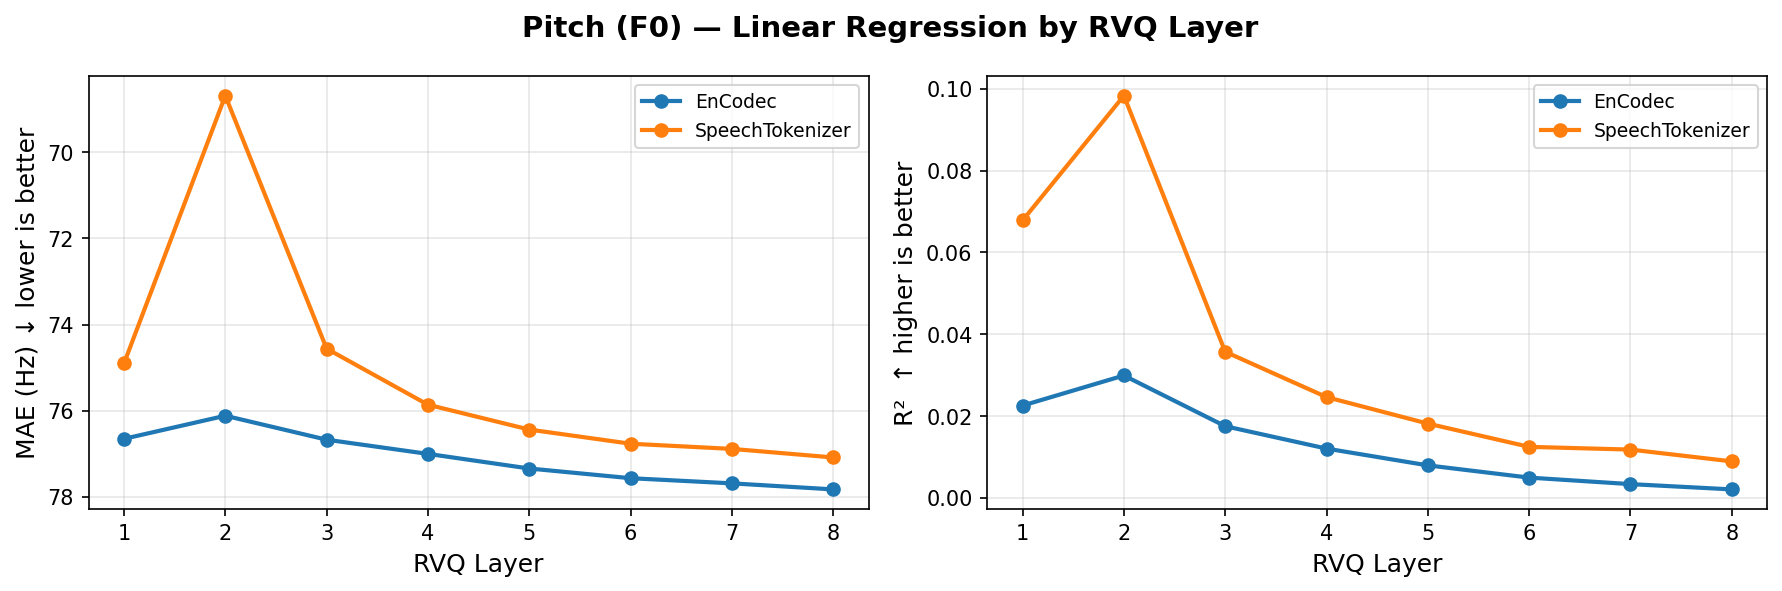
\includegraphics[width=\textwidth]{remoteA100/pitch_probing.png}
  \caption{Pitch (F0) linear regression results by RVQ layer.
           \emph{Left:} MAE in Hz (lower is better; $y$-axis inverted).
           \emph{Right:} $R^2$ (higher is better).
           Both codecs achieve low $R^2$ ($<$0.10), indicating that
           fundamental frequency is not well linearly decodable from
           discrete RVQ embeddings. SpeechTokenizer peaks at Layer~2
           ($R^2$\,=\,0.098), mirroring the speaker identity pattern.}
  \label{fig:pitch}
\end{figure*}

% ── t-SNE Figures ─────────────────────────────────────────────────────────────
\begin{figure*}[t]
  \centering
  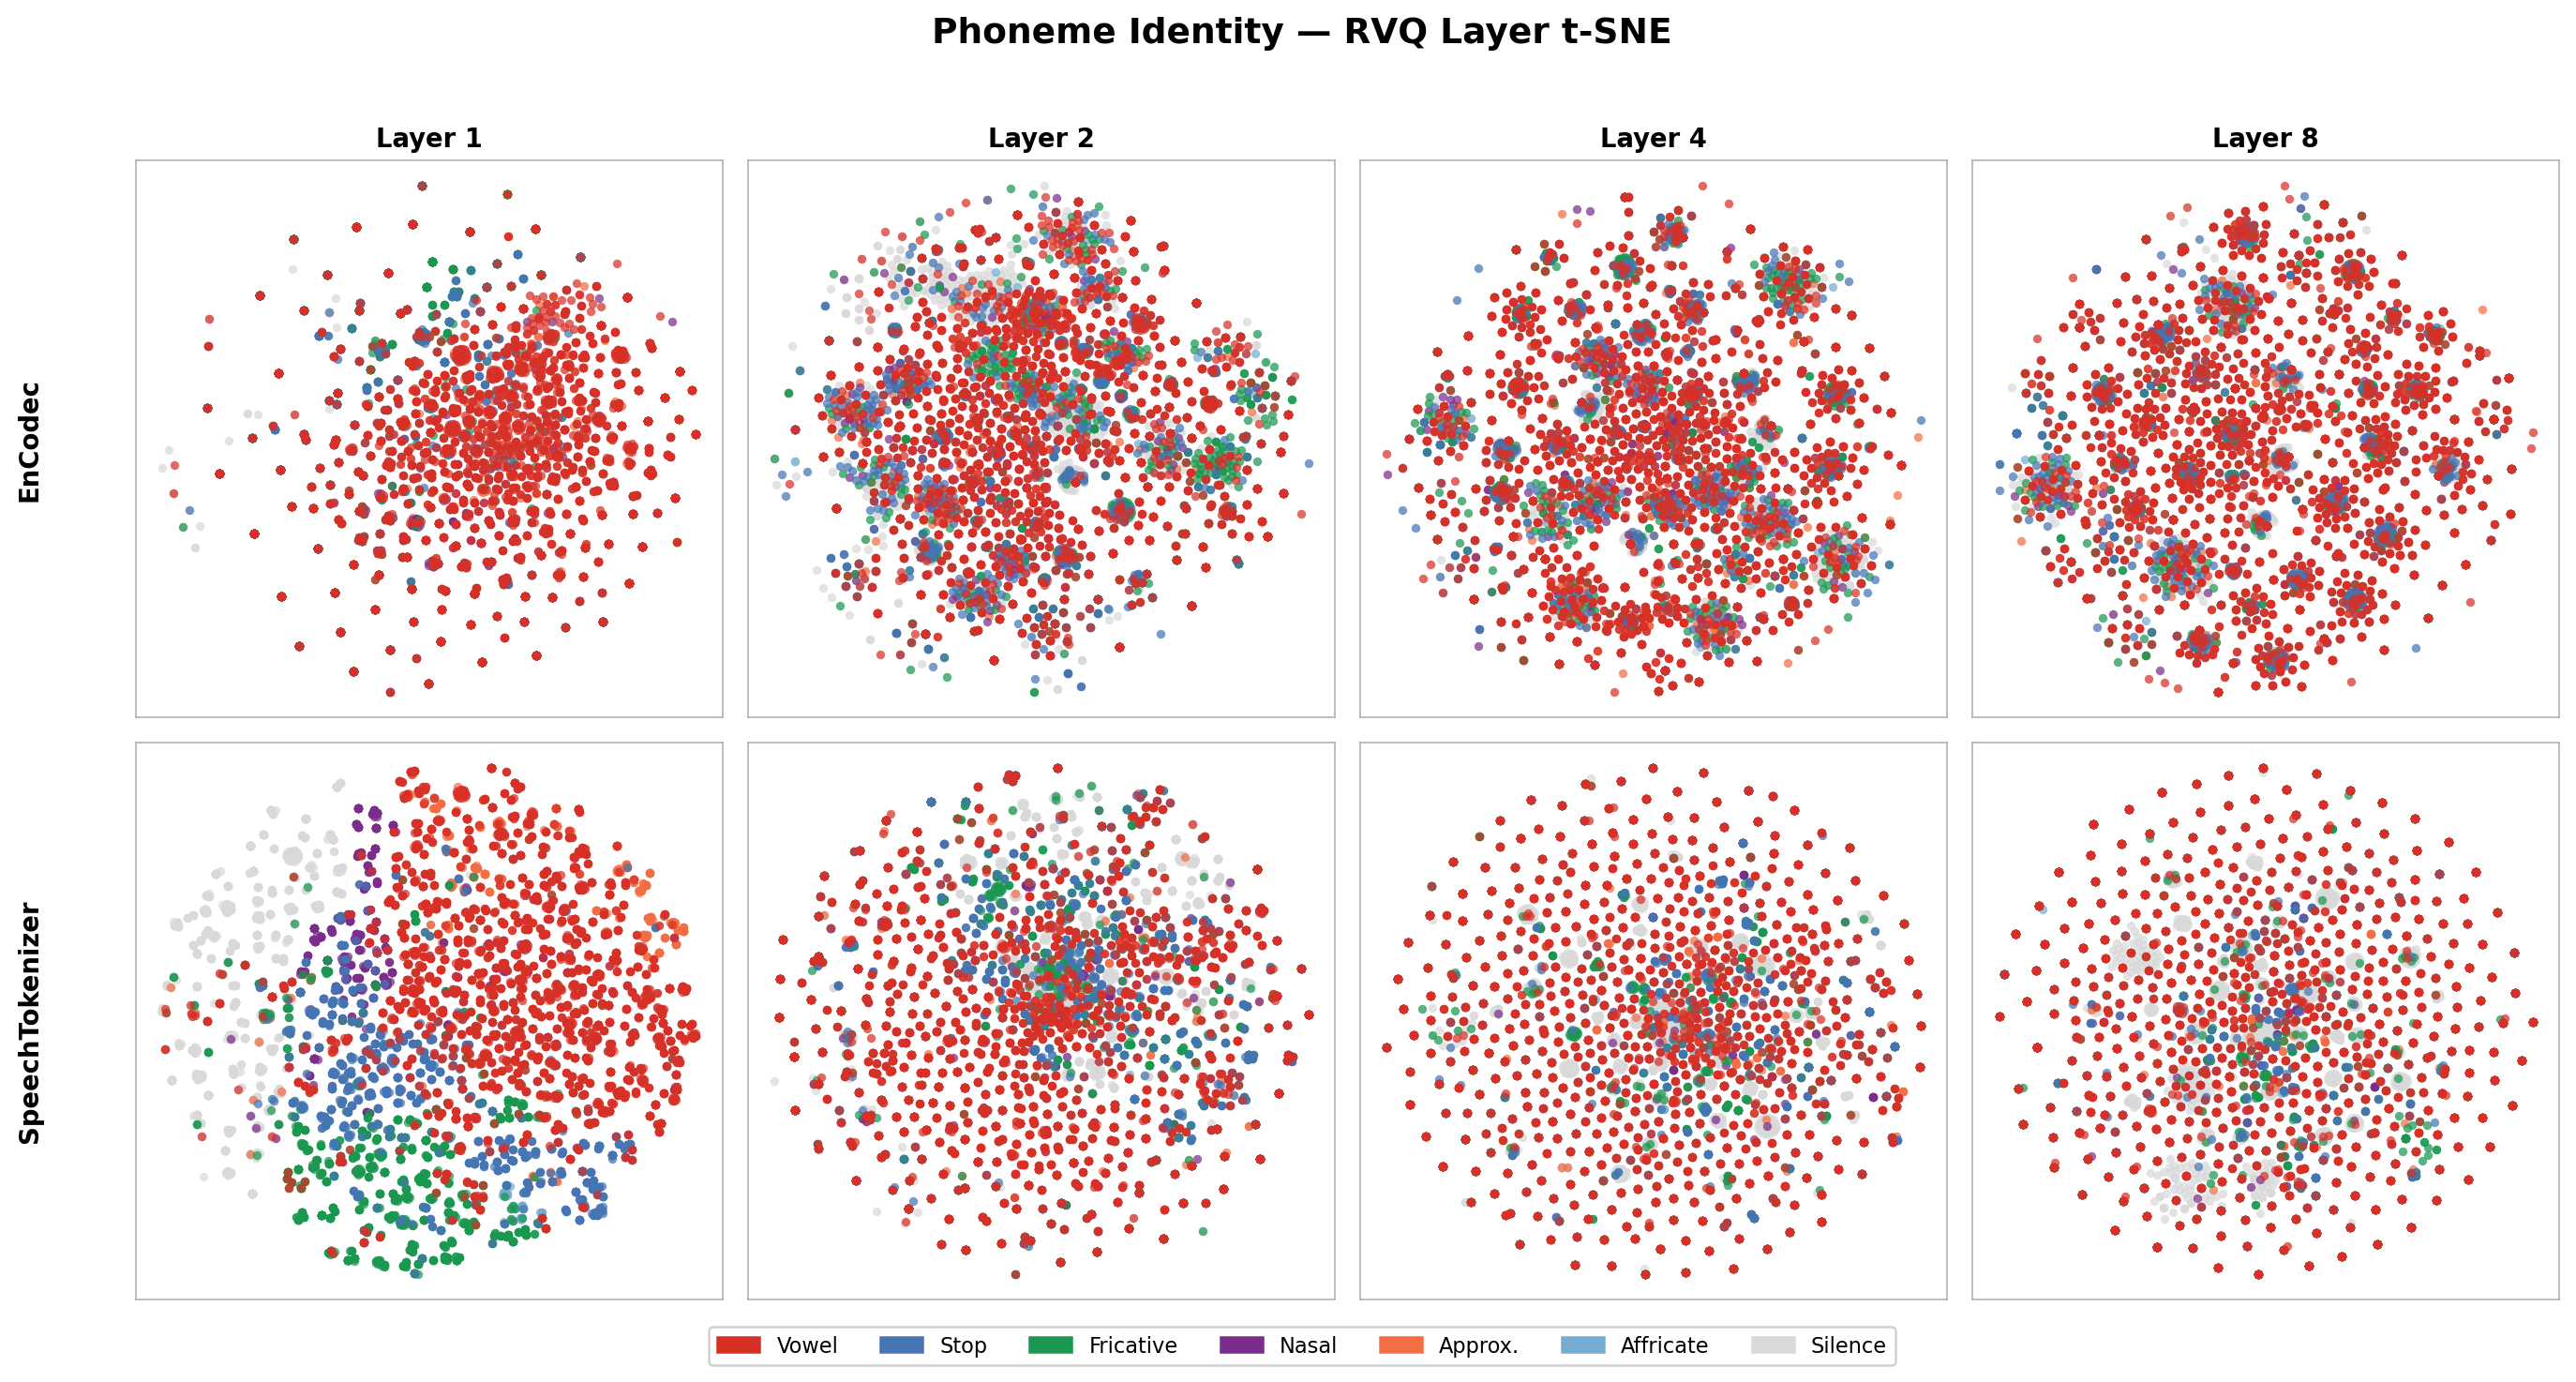
\includegraphics[width=\textwidth]{remoteA100/tsne_phoneme.png}
  \caption{t-SNE projection of codec token embeddings colored by phoneme group
           (rows\,=\,codecs; columns\,=\,RVQ layers 1, 2, 4, 8).
           SpeechTokenizer Layer~1 (top-right) shows appreciably tighter
           phoneme-group clusters---especially for vowels (red) and stops
           (blue)---compared to EnCodec Layer~1 (top-left), corroborating
           the 9$\times$ macro-F1 gap in Figure~\ref{fig:phoneme}.
           Clustering weakens progressively in later layers for both codecs.}
  \label{fig:tsne_phoneme}
\end{figure*}

\begin{figure*}[t]
  \centering
  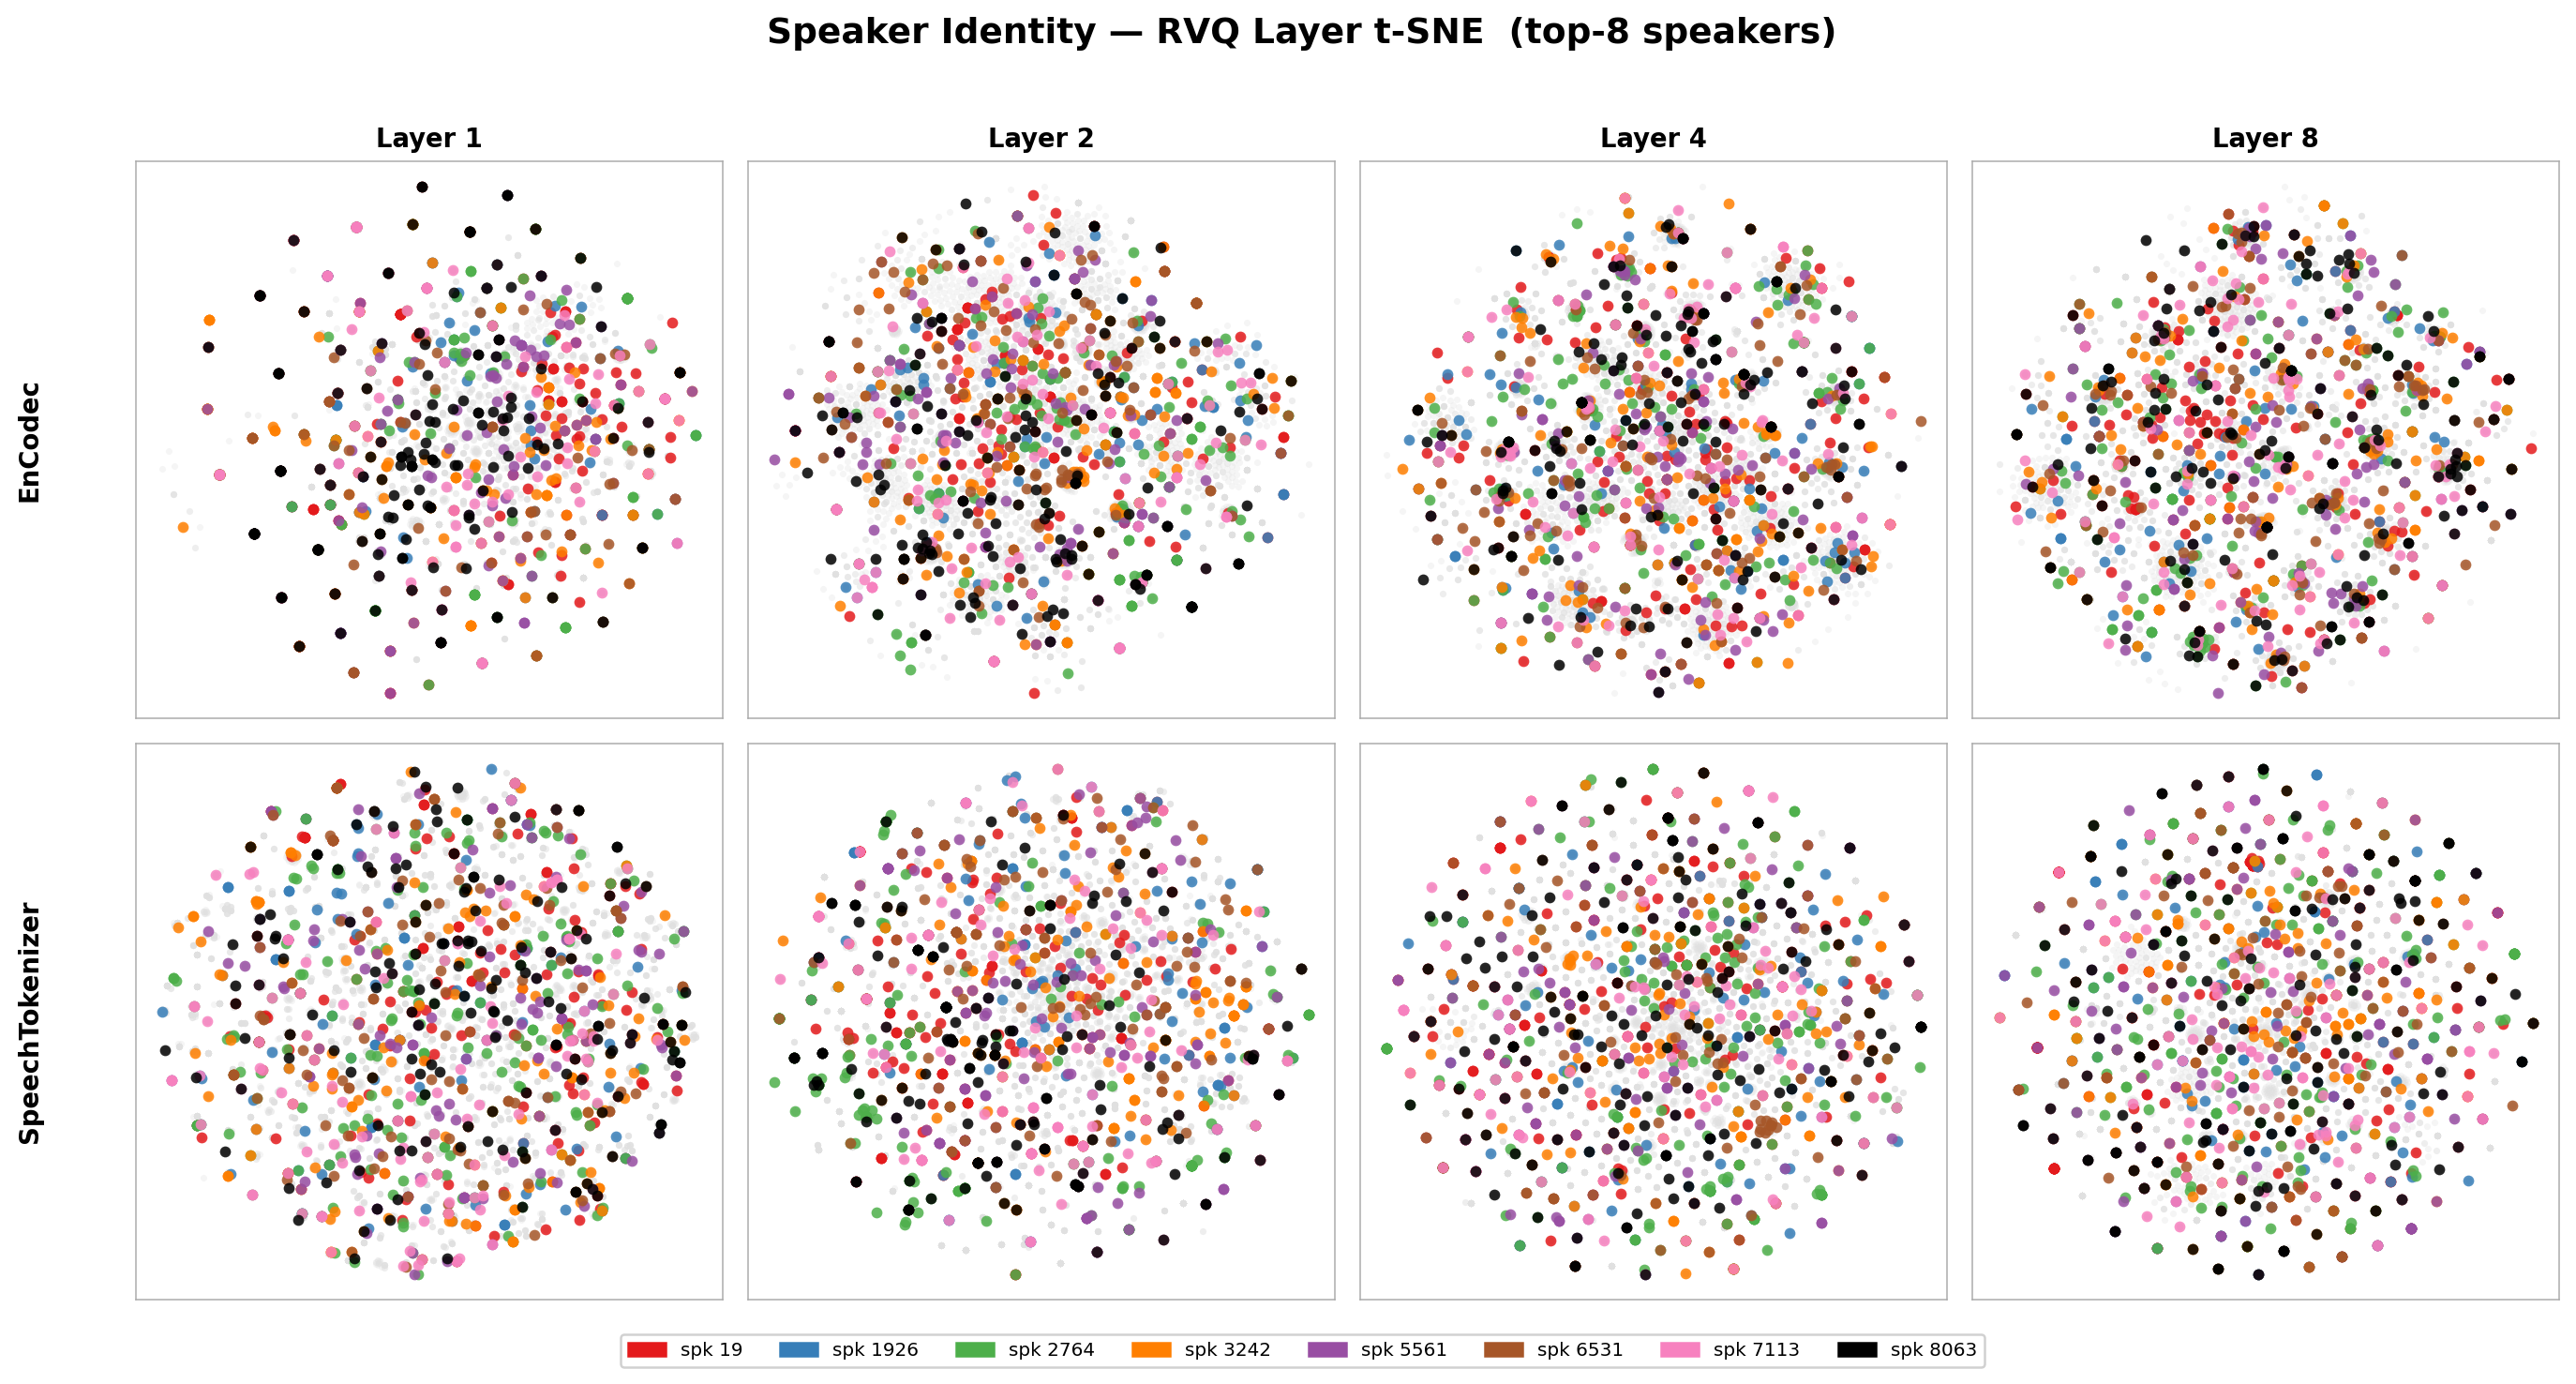
\includegraphics[width=\textwidth]{remoteA100/tsne_speaker.png}
  \caption{t-SNE projection colored by speaker identity. The top-8 most
           frequent speakers are highlighted in distinct colors; remaining
           speakers appear in light gray. Neither codec produces strongly
           separated speaker clusters at any layer, consistent with the
           low absolute macro-F1 scores ($<\!0.05$). SpeechTokenizer
           Layer~2 shows marginally more per-speaker spatial cohesion
           than Layer~1, reflecting the Layer~2 peak in
           Figure~\ref{fig:speaker}.}
  \label{fig:tsne_speaker}
\end{figure*}

\begin{figure*}[t]
  \centering
  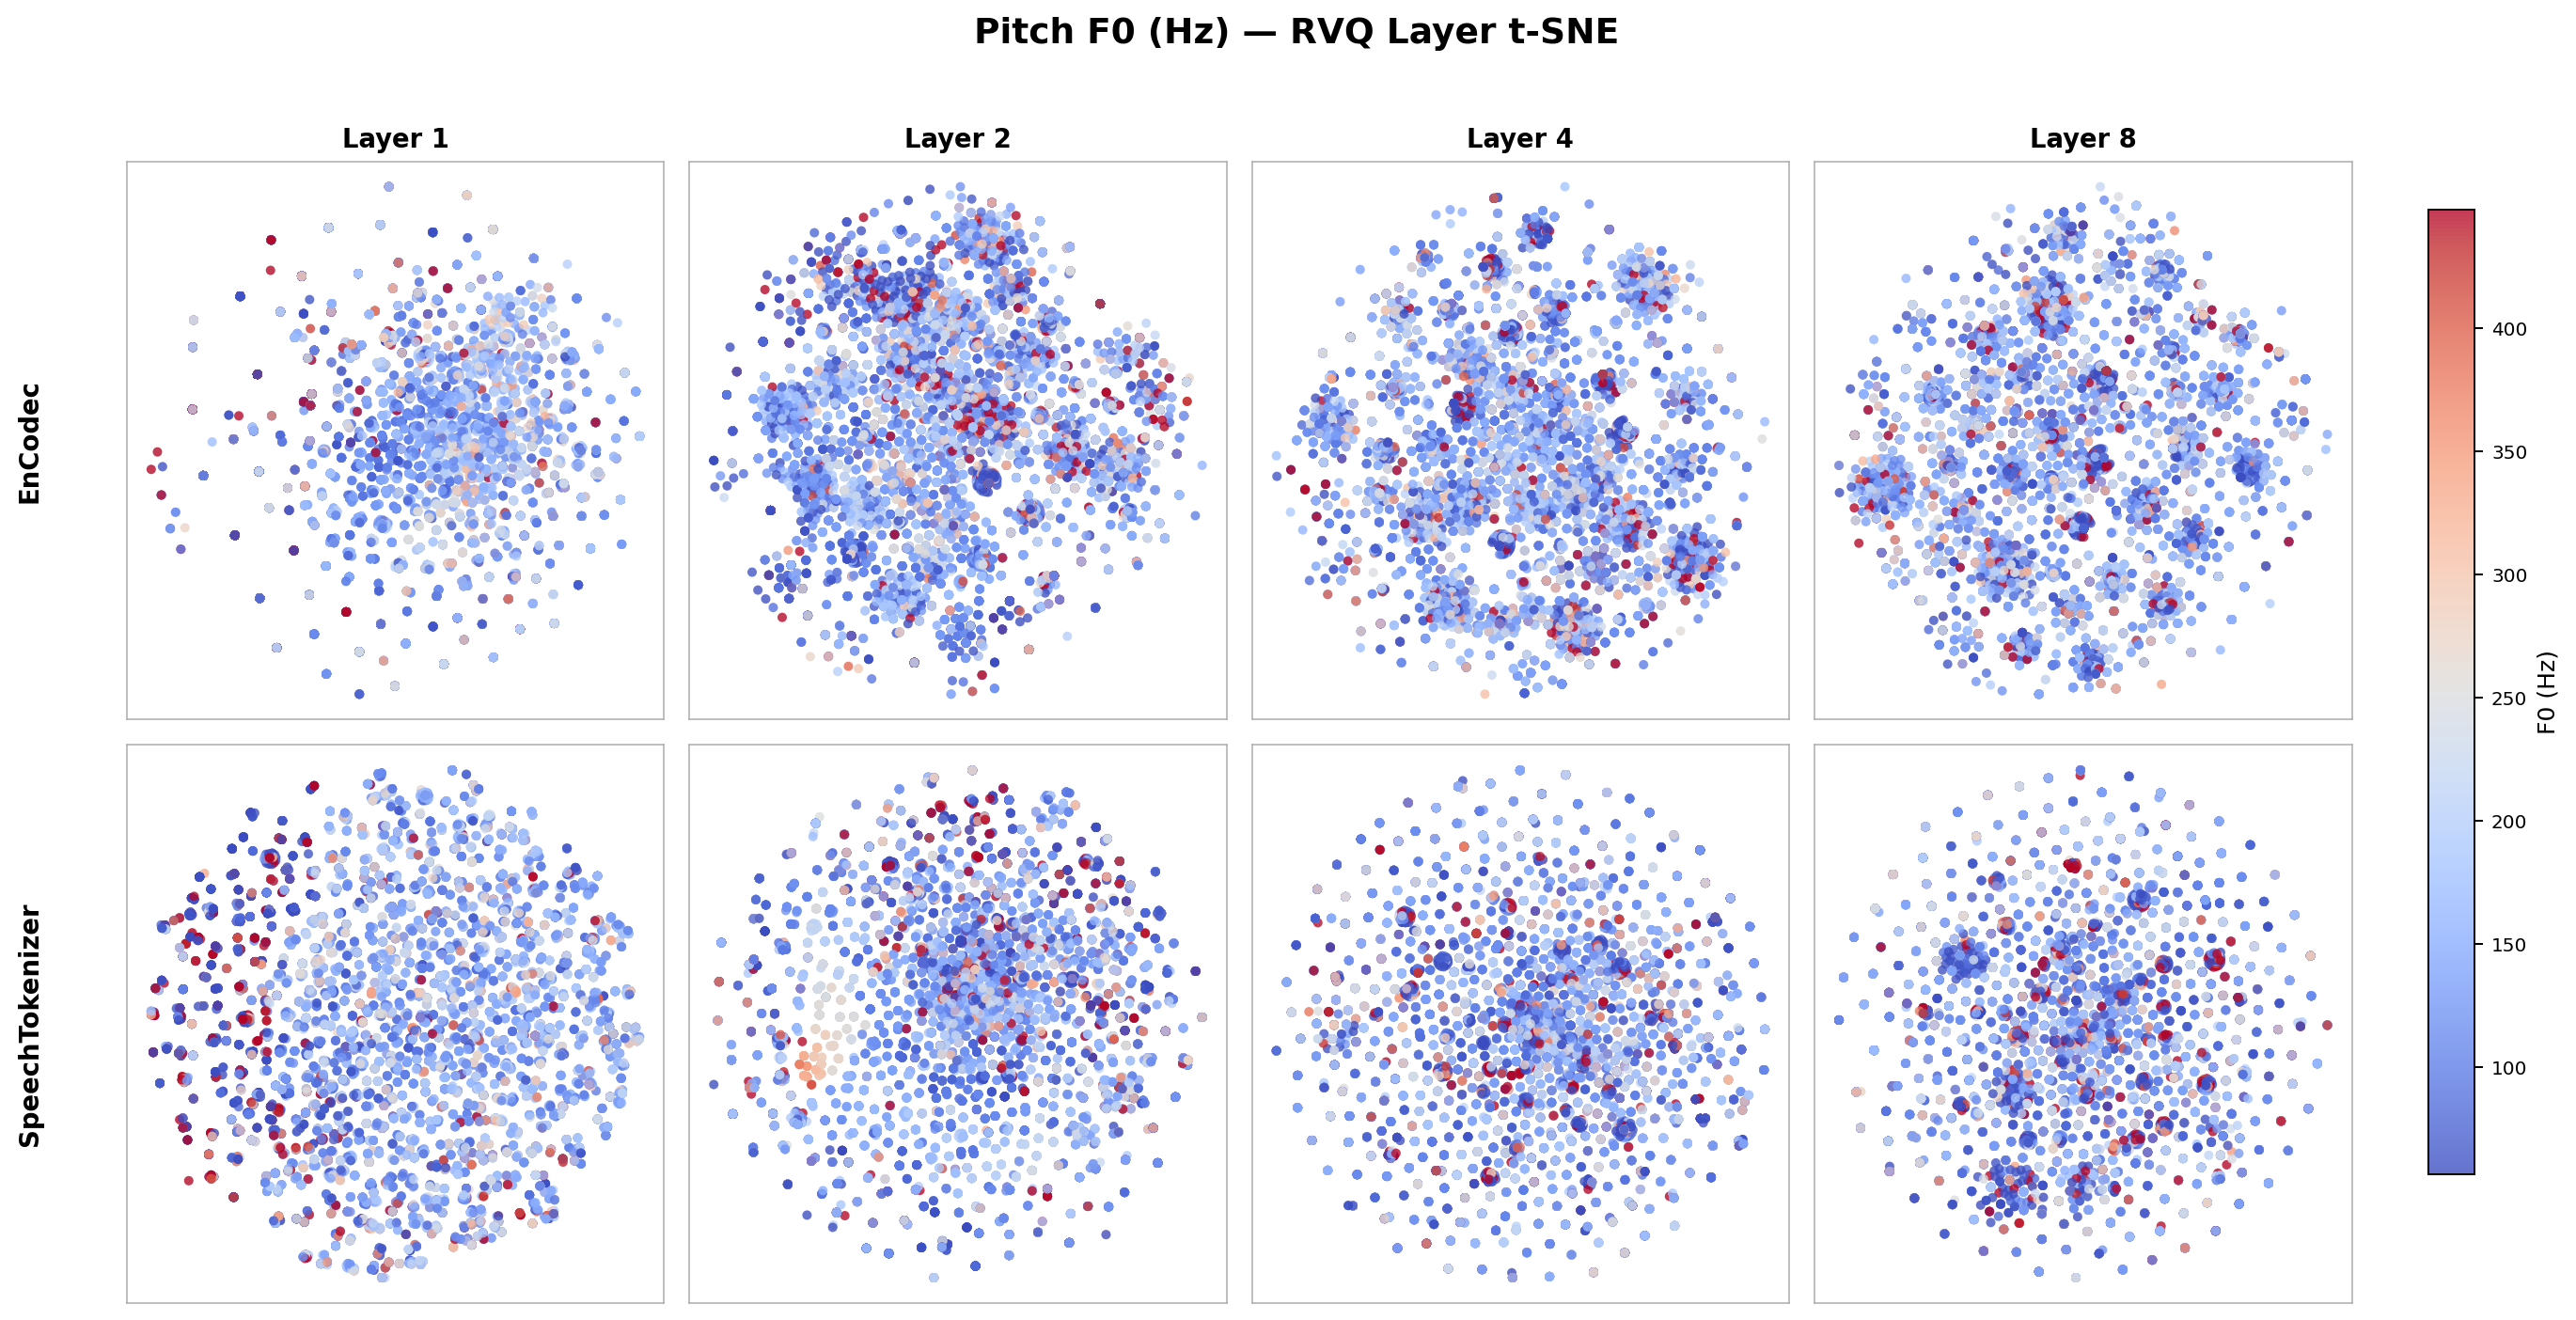
\includegraphics[width=\textwidth]{remoteA100/tsne_pitch.png}
  \caption{t-SNE projection colored by fundamental frequency F0
           (coolwarm colormap: blue\,=\,low pitch, red\,=\,high pitch).
           Unvoiced tokens are shown in light gray.
           No systematic spatial pitch gradient is visible in either
           codec at any layer, consistent with $R^2\,{<}\,0.10$
           throughout (Figure~\ref{fig:pitch}).}
  \label{fig:tsne_pitch}
\end{figure*}

% ── 5. Future Work ────────────────────────────────────────────────────────────
\section{Future Work}

Several natural extensions follow from this work.

\paragraph{Non-linear probes.}
Linear probes reveal whether a concept is explicitly encoded in a
linear-separable form, but they cannot detect information that is
present but non-linearly organized. Training shallow MLP probes (one or
two hidden layers) on the same embeddings would reveal whether EnCodec's
near-random phoneme scores reflect true information absence or
non-linear entanglement. If MLP probes recover substantially higher
phoneme accuracy for EnCodec, it would suggest that phoneme information
is implicit but extractable, with implications for codec-based speech LM
design.

\paragraph{Full token budget.}
This study was constrained to 50,000 training tokens per probe due to
memory limitations. Running probes on the full available training corpus
(16--24 million tokens) would provide more reliable accuracy estimates,
particularly for rare phoneme classes and speakers. With sufficient
compute, the full lbfgs optimization should converge within EnCodec's
128-dimensional embedding space.

\paragraph{Additional linguistic properties.}
The three tasks studied here (phoneme, speaker, pitch) are the most
commonly used in speech probing work, but other properties merit
investigation: \emph{emotion}, \emph{speaking rate}, \emph{signal-to-noise
ratio}, \emph{accent}, and \emph{word-level stress}. Multi-label probing
could also reveal whether individual RVQ codes are jointly predictive
of multiple attributes simultaneously.

\paragraph{Probing codec token indices vs.\ embeddings.}
The present study probes the continuous quantized embedding vectors
output by each RVQ codebook. An equally interesting question is whether
the discrete \emph{indices} (the token IDs used by speech LMs) encode
the same structure. Mutual information between token index sequences and
phoneme sequences would directly characterize what an autoregressive
language model ``sees'' when operating on codec tokens.

\paragraph{Other codecs.}
The linear probing framework developed here is directly applicable to
other recent codecs such as DAC~\cite{kumar2023} and
Mimi~\cite{defossez2024}, enabling a broader comparative study of how
architectural and training choices affect representational structure.

% ── 6. Conclusion ─────────────────────────────────────────────────────────────
\section{Conclusion}

We have presented the first systematic linear probing study comparing
EnCodec and SpeechTokenizer across all 8 RVQ layers and three
linguistically meaningful tasks: phoneme identity, speaker identity,
and pitch. Our results provide quantitative confirmation of the
layer-specialization hypothesis in SpeechTokenizer: its first RVQ
layer, trained with semantic distillation from HuBERT, achieves a
phoneme macro-F1 of 0.338, nine times higher than EnCodec's best
layer. Speaker information peaks at SpeechTokenizer's Layer~2, not
Layer~1, revealing that the semantic/acoustic factorization induced by
the training objective extends to paralinguistic properties. Pitch
remains poorly accessible from linear read-outs of either codec's
embeddings, highlighting the information loss inherent in discrete
quantization for continuous prosodic features.

These findings have practical implications for the design of
codec-based speech language models. SpeechTokenizer's explicit semantic
layer provides a cleaner factorization that may simplify downstream
models: semantic (phoneme-level) decisions can be made using Layer~1
alone, while speaker and prosodic conditioning can be applied through
later layers. EnCodec's lack of layer specialization places a heavier
burden on the downstream model to disentangle these properties
implicitly.

More broadly, this work demonstrates that linear probing---a tool
borrowed from the NLP interpretability literature---is directly
applicable to discrete speech codec representations and yields
interpretable, quantitative insights about their structure.

% ── References ────────────────────────────────────────────────────────────────
\clearpage
\bibliographystyle{plain}

\begin{thebibliography}{10}

\bibitem{alain2016}
G.~Alain and Y.~Bengio.
\newblock Understanding intermediate layers using linear classifier probes.
\newblock In \emph{ICLR Workshop}, 2017.
\newblock arXiv:1610.01644.

\bibitem{conneau2018}
A.~Conneau, G.~Kruszewski, G.~Lample, L.~Barrault, and M.~Baroni.
\newblock What you can cram into a single vector: Probing sentence embeddings
  for linguistic properties.
\newblock In \emph{Proceedings of ACL}, 2018.

\bibitem{defossez2023}
A.~D{\'e}fossez, J.~Copet, G.~Synnaeve, and Y.~Adi.
\newblock High fidelity neural audio compression.
\newblock \emph{Transactions on Machine Learning Research}, 2023.

\bibitem{defossez2024}
A.~D{\'e}fossez et al.
\newblock Moshi: A speech-text foundation model for real-time dialogue.
\newblock arXiv:2410.00037, 2024.

\bibitem{hsu2021}
W.-N. Hsu, B.~Bolte, Y.-H.~H. Tsai, K.~Lakhotia, R.~Salakhutdinov, and
  A.~Mohamed.
\newblock {HuBERT}: Self-supervised speech representation learning by masked
  prediction of hidden units.
\newblock \emph{IEEE/ACM Transactions on Audio, Speech, and Language
  Processing}, 29:3451--3460, 2021.

\bibitem{kumar2023}
R.~Kumar, P.~Seetharaman, A.~Luebs, I.~Kumar, and K.~Kumar.
\newblock High-fidelity audio compression with improved {RVQGAN}.
\newblock In \emph{Advances in Neural Information Processing Systems
  (NeurIPS)}, 2023.

\bibitem{mcauliffe2017}
M.~McAuliffe, M.~Socolof, S.~Mihuc, M.~Wagner, and M.~Sonderegger.
\newblock Montreal forced aligner: Trainable text-speech alignment using
  {Kaldi}.
\newblock In \emph{Interspeech}, 2017.

\bibitem{panayotov2015}
V.~Panayotov, G.~Chen, D.~Povey, and S.~Khudanpur.
\newblock {LibriSpeech}: An {ASR} corpus based on public domain audio books.
\newblock In \emph{IEEE International Conference on Acoustics, Speech and
  Signal Processing (ICASSP)}, 2015.

\bibitem{rubenstein2023}
P.~K. Rubenstein et al.
\newblock {AudioPaLM}: A large language model that can speak and listen.
\newblock arXiv:2306.12925, 2023.

\bibitem{sadok2025}
S.~Sadok, J.~Hauret, and É.~Bavu.
\newblock Bringing Interpretability to Neural Audio Codecs.
\newblock In \emph{Interspeech}, 2025.

\bibitem{sklearn}
F.~Pedregosa et al.
\newblock Scikit-learn: Machine learning in {Python}.
\newblock \emph{Journal of Machine Learning Research}, 12:2825--2830, 2011.

\bibitem{wang2023}
C.~Wang et al.
\newblock {VALL-E}: Neural codec language models are zero-shot text to speech
  synthesizers.
\newblock arXiv:2301.02111, 2023.

\bibitem{zhang2024}
X.~Zhang et al.
\newblock {SpeechTokenizer}: Unified speech tokenizer for speech language
  models.
\newblock In \emph{International Conference on Learning Representations
  (ICLR)}, 2024.

\end{thebibliography}

\end{document}
